L'algorithme de Ruppert permet de remplir (trianguler) une forme définie par un ensemble de segments (lui même constitué d'un ensemble de points). Les triangles ainsi formés respectent une certaine qualité définie par l'utilisateur: chaque triangle de la triangulation
finale devra avoir son plus petit angle supérieur à un seuil donné.

L'algorithme fonctionne en plusieurs étapes:
\begin {itemize}
	\item {On commence par créer une triangulation de Delaunay (Lawson incrémental) à partir des points donné en entrée à l'algorithme}
	\item {Une fois la triangulation obtenue, on vérifie que tous les segments de notre forme de départ font bien partie de notre triangulation.}
	\item {Pour chaque segment de la forme de départ qui ne fait pas partie de la triangulation, on insère un nouveau sommet au centre du segment, produisant deux nouveaux segments}
	\item {Si le segment ne fait toujours pas partie de la triangulation, on continue à découper récursivement les nouveaux segments}
	\item {Une fois tous les segments inclus dans la triangulation, on va insérer des nouveaux sommets au centre des cercles circonscrits aux triangles qui ne respectent par le seuil sur les angles donné. Le sommet est inséré au centre du triangle si et seulement si le sommet a insérer ne tombe pas dans le cercle diamétral d'un des segments de contrainte.}
	\item {Le résultat est une triangulation de Delaunay avec une garantie de qualité (seuil sur les angle des triangles) qui contient tous les segments de la forme de départ.}
\end {itemize}

\begin{figure}[h!]
	\adjustbox{center}{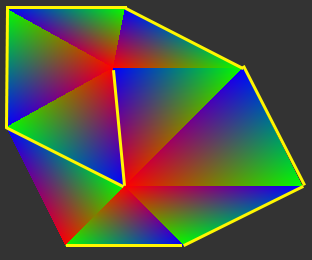
\includegraphics[width=0.6\textwidth]{Captures/RuppertSegments.png}}
	
	\caption{Les segments de contraintes sont représentés en jaune. L'algorithme de Ruppert permet de trianguler la forme.}
\end{figure}
\FloatBarrier
